\section{Théorie}
% La viscosité d'un fluide à une température donnée $\eta$ correspond à sa capacité à amortir, ou diminuer, les déplacements du fluide. Dans le cas de l'expérience simple présentée en \autoref{fig:plaques} avec deux plaques séparées par un fluide dont l'une est maintenue immobile et l'autre est déplacée à vitesse constante $\vec{v}_t$ cela donne:
% \begin{equation}
%     \vec{F}_t = \eta \frac{S\vec{v}_t}{e}
% \end{equation} 
% avec $\vec{F}_t$ la force appliquée, $S$ la surface de la plaque et $e$ la distance entre les deux plaques. Il est aussi utilde de définir la viscosité cinématique: $\nu = \eta/\rho$.

% \begin{figure}[h]
%     \centering
%     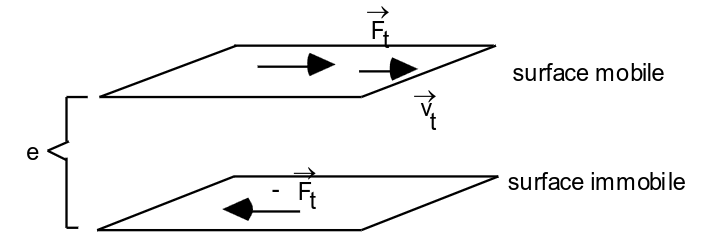
\includegraphics[width=0.6\linewidth]{figures/viscosite_plaques.png}
%     \caption{Expérience permettant de mesurer la viscosité d'un liquide \cite{notice}}
%     \label{fig:plaques}
% \end{figure}

Lorsqu'un solide se déplace dans un fluide la même viscosité va donner lieu à une force de traînée dans la direction du mouvement et dans le sens opposé et dont la norme s'exprime dans le cadre général sous la forme:
\begin{equation}
    T = C_x S \frac{1}{2} \rho v_\infty ^2
    \label{eq:trainee_gen}
\end{equation}
avec $S$ la surface de projection de l'obstacle, $\rho$ la densité du fluide concerné et \(v_\infty ^2\) la vitesse par rapport au fluide loin de l'obstacle. Le coefficient $C_x$ quant à lui est bien plus difficile à déterminer et est dans la majorité des cas empirique. Il dépend cependant du nombre de Reynold lui-même dépendant de la viscosité par définition:
\begin{equation}
    \mathrm{Re} = \frac{\rho}{\eta}v_\infty L
    \label{eq:Reynolds}
\end{equation}
avec $L$ une grandeur caractéristique du solide, par exemple le diamètre pour une sphère.

Il est possible d'utiliser la formule de Stokes pour l'intervalle $0 \leq \mathrm{Re} \leq 0.5$ qui donne \hbox{$C_x = 24/\mathrm{Re}$}. Pour une sphère de rayon $r$ cela permet d'obtenir à partir de l'\autoref{eq:trainee_gen}:
\begin{equation}
    T = 6 \pi \eta r v_\infty
    \label{eq:trainee_stokes}
\end{equation}

Le cas étudié ici sera celui où la bille a atteint sa vitesse maximale pendant sa chute dans le champ de gravité $\vec{g}$ correspondant donc à un équilibre des forces présentes, la traînée, le poids de la bille de masse $m$ ($m\vec{g}$) et la poussée d'Archimède ($4/3 \pi r^3 \rho \vec{g}$). Ainsi il est possible d'obtenir une formule pour la viscosité:
\begin{equation}
    \eta = \frac{g(m-\frac{4}{3}\pi r^3 \rho)}{6\pi r v_\infty}
    \label{eq:viscosite}
\end{equation}

La fluidité $1/\eta$ dépend d'une relation de Boltzmann ce qui permet d'obtenir une relation entre la viscosité et la température $T$ du liquide. Cela s'exprime par:
\begin{equation}
    \frac{1}{\eta} = \frac{1}{A} \exp\left(-\frac{E}{k_b T}\right)
\end{equation}
\begin{equation}
    \Rightarrow \ln(\eta) = \ln(A) + \frac{E}{k_b T}
    \label{eq:ln_relation_boltzmann}
\end{equation}
avec $k_b = 1.38 \times 10^{-23}$ la constante de Boltzmann, $1/A$ la fluidité quand $T \to \infty$ et $E$ une énergie d'activation. Cela permet de déduire que $\ln(\eta)$ dépend linéairement de $1/T$.

La dernière analyse nécessaire pour plus tard vérifier la cohérence de nos mesures est le temps mis par la bille pour atteindre sa vitesse d'équilibre. La trainée en fonction du temps est donnée par l'expression $T(t) = 6\pi \eta r v(t)$ avec $v$ la vitesse. Cela permet d'obtenir avec les deux autres forces constantes l'équation différentielle suivante pour la position $x$:
\begin{equation}
    \ddot{x} = \frac{1}{m}(mg - 6\pi \eta r \dot{x} - \rho V g)
\end{equation}
où le volume de la bille est noté $V = 4/3 \pi r^3$. En posant $\alpha = -6\pi \eta r / m$, $\beta = g(1-\rho V/m)$ et $X = \dot{x}$ cela donne $\dot{X} = \alpha X + \beta$. En résolvant cette équation différentielle cela donne la solution pour la condition initiale $v(t=0)=0$:
\begin{equation}
    \dot{x}(t) = X = \frac{\beta}{\alpha}(e^{\alpha t} - 1)
\end{equation}
Ainsi la vitesse tend avec une décroissance exponentielle vers une vitesse de $\beta/\alpha$. Cette décroissance exponentielle à la forme $\exp(-t/\tau)$ avec $\tau$ une constante de temps qui s'exprime:
\begin{equation}
    \tau = -\frac{1}{\alpha} = \frac{m}{6\pi \eta r}
    \label{eq:constante_temps}
\end{equation}
